\chapter{Resultados}\label{cap:10resultados}

Este capítulo pone fin al desarrollo teórico-práctico del proyecto, realizando una recopilación de los resultados obtenidos durante el mismo. A continuación se listan los resultados obtenidos:

\begin{itemize}

    \item \textbf{Res-001: Conocimiento y participación activa en la comunidad de OHDSI.} Al término del proyecto, se ha obtenido un conocimiento teórico exhaustivo de OHDSI, de sus estándares y sus herramientas y por supuesto de la herramienta ATLAS en todos sus aspectos, tal y como se detalla en los aspectos teóricos del trabajo.
    
    Sin embargo, lo más importante de haber conocido y comprendido la organización Observational Health Data Sciences and Informatics ha sido entender la importancia de la participación colaborativa en la comunidad, que he realizado mediante la participación en foros de la comunidad \parencite{OHDSIforums} y formando parte de los grupos de Discord \parencite{OHDSIdiscordInvitation} y MS Teams de la comunidad. Mi proyecto termina pero el camino con OHDSI (\textit{''the journey''}) todavía continúa.
    
    \item \textbf{Res-002: Aplicación y redacción del manual de despliegue de ATLAS Broadsea.} Frente a todos los problemas encontrados durante la instalación, despliegue y configuración de ATLAS Broadsea, haber dejado por escrito una guía detallada del proceso es uno de los resultados más destacables del proyecto, por la relevancia que tendrá para el resto de investigadores poder poseer de un manual sencillo que comprenda todos los conocimientos teóricos y prácticos necesarios para realizar esta tarea.

    Además, por la naturaleza práctica del proyecto realizado en colaboración con el HUVR, el interés de este manual es aún mayor, pues les facilitará enormemente realizar esta tarea si la requiriesen una vez cese mi periodo de prácticas. 

    \item \textbf{Res-003: Desarrollo de un estudio reproducible a través de ATLAS y el repositorio de github.} Por último, la utilización de ATLAS para demostrar la viabilidad de la herramienta a la hora de conducir estudios de análisis de datos de forma sencilla, a través de guías de buenas prácticas y múltiples tutoriales online ha sido un resultado muy importante. 

    Sin embargo, lo más destacable del caso práctico no ha sido solo la facilidad con la que se ha podido reproducir el estudio sino la facilidad para generar código exportable a partir del mismo y compartirlo en el repositorio de github del proyecto, alineando el TFG a la visión o\textit{pen-source} y \textit{open-science} de la comunidad de OHDSI. 

\end{itemize}

\section{Trazabilidad de objetivos}

Los resultados obtenidos durante el proyecto casan con los objetivos definidos en el capítulo \ref{cap:02objetivos} ''Objetivos del Proyecto''. 

A continuación se muestra una tabla que señala los objetivos que satisface cada uno de los resultados obtenidos. Se contemplan los objetivos del proyecto y los objetivos personales de la alumna.

\begin{figure}[H]
    \centering
    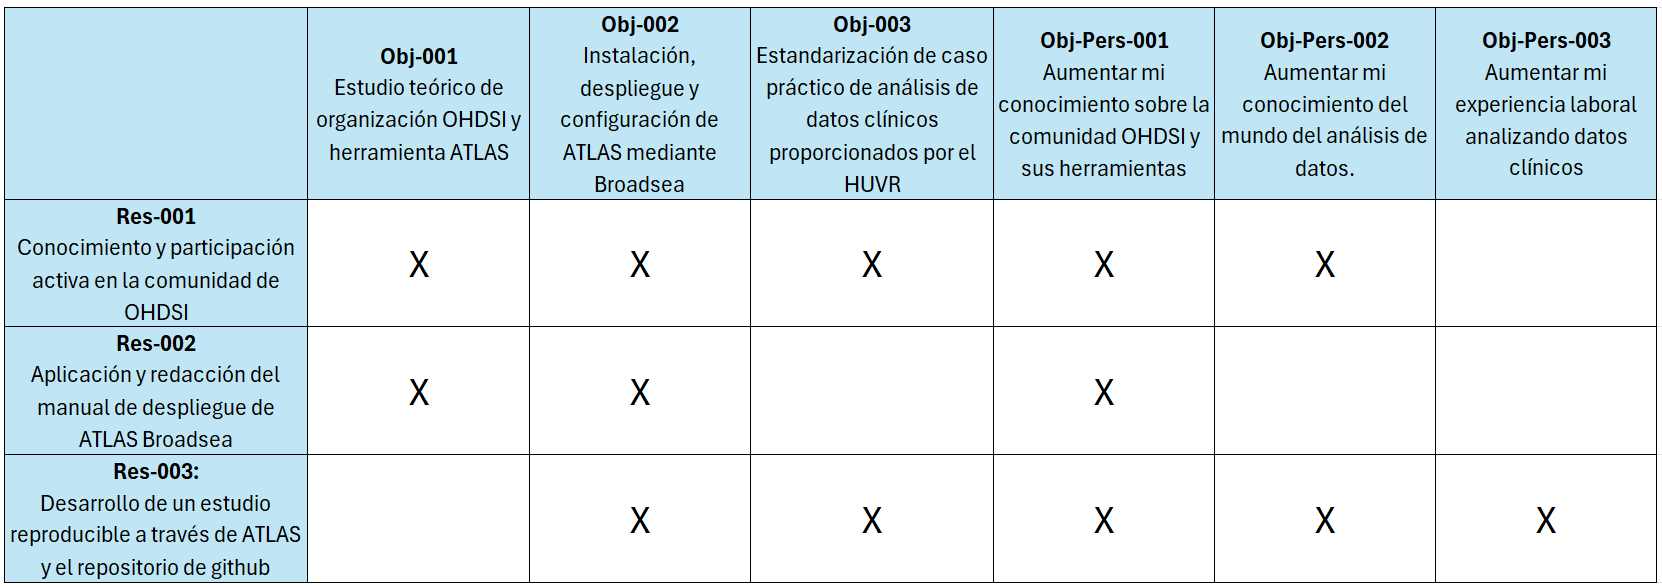
\includegraphics[width=1\textwidth]{tables/trazabilidadObjetivosPers.png}
    \captionof{table}{Trazabilidad de objetivos con resultados}
    \label{table:trazabilidadObjetivosPers}
\end{figure}

%Como muestra la tabla anterior, todos los objetivos quedan satisfechos al menos por un resultado. 

\begin{itemize}
    \item \textbf{Trazabilidad del Res-001.} Este resultado abarca prácticamente todos los objetivos, puesto que el conocimiento teórico de la organización es subyacente a cada paso en la elaboración del proyecto, tanto en la teoría como en la práctica, haciendo especial hincapié en la parte práctica a la hora de participar en los foros de la comunidad publicando y revisando preguntas sobre las herramientas empleadas durante el desarrollo del proyecto.
    \item \textbf{Trazabilidad del Res-002.} Este resultado abarca objetivos de aspecto teórico y de implementación. No se considera que contribuya a los objetivos de análisis porque realiza más bien las tareas de desarrollador, montando la estructura Docker y la base de datos del sistema (véase \ref{cap:07entorno} ''Entorno de Trabajo''). El estudio teórico de OHDSI ha sido fundamental para poder implementar correctamente el sistema.
    \item \textbf{Trazabilidad del Res-003.} Este resultado abarca los objetivos relacionados con el análisis y con la herramienta de ATLAS Broadsea, que al fin y al cabo es la que se ha utilizado para llevar a cabo el análisis. Además del análisis, el repositorio de github también recopila archivos importantes y documentación del manual por lo que también se relaciona con este objetivo.
\end{itemize}


\section{Lecciones aprendidas}

Este proyecto ha sido de gran relevancia para culminar mi formación académica y dar inicio a mi carrera profesional, permitiéndome aplicar los conocimientos adquiridos en el Grado de Ingeniería de la Salud y abriendo nuevas oportunidades en el ámbito del tratamiento de datos clínicos. La integración de teoría y práctica en este proyecto ha sido fundamental para mi desarrollo como profesional en esta disciplina.

La lección más significativa que he obtenido de este proyecto es \textbf{la importancia de aprender de los errores y ser capaz de enfrentar y resolver problemas inesperados}. Esta habilidad es esencial para cualquier ingeniero, ya que los desafíos imprevistos son comunes en el ámbito profesional y académico.

Aprender a desplegar y utilizar ATLAS de manera autodidacta ha sido un reto sumamente valioso. Este proceso no solo implicó una investigación exhaustiva para comprender el funcionamiento de la herramienta y sus configuraciones, sino también una inmersión en el ecosistema de herramientas y estándares de OHDSI. Esta experiencia me ha formado como una experta en el campo, destacando la importancia de la investigación independiente y el autoaprendizaje en el desarrollo profesional.

Estos conocimientos teóricos me han permitido comprender la necesidad crítica de la interoperabilidad entre los sistemas de información, especialmente en el ámbito sanitario, y los desafíos y limitaciones que esto implica. Reconozco la labor crucial que realiza OHDSI para estandarizar la investigación clínica, subrayando su relevancia a nivel mundial y europeo. Aunque actualmente OHDSI no es el estándar predominante, estoy convencida de que lo será en el futuro, y los conocimientos adquiridos ahora serán aún más valiosos en los próximos años.

Gracias a todo lo aprendido, actualmente colaboro con el grupo de Informática de la Salud del HUVR en el proyecto europeo IMPaCT-Data. En este proyecto, he contribuido a la redacción de secciones que proponen soluciones relacionadas con OHDSI, el Modelo de Datos Común de OMOP y ATLAS. Esta colaboración ha sido una oportunidad invaluable para aplicar mis conocimientos en un contexto real y contribuir a un proyecto de gran impacto.

La colaboración con el HUVR y con Francisco Rey Garduño, en relación con nuestros Trabajos de Fin de Grado, me han enseñado mucho sobre el trabajo en equipo, la importancia de la distribución de tareas, la planificación del tiempo y la asunción de responsabilidades. Estas habilidades son esenciales para el éxito en cualquier proyecto profesional.

Desde una perspectiva práctica, el despliegue de ATLAS me ha aportado nuevos conocimientos sobre Docker y ha mejorado mis habilidades en bases de datos. Nunca había trabajado con Docker antes de este proyecto, y aprender sobre la configuración de contenedores y perfiles, la identificación y resolución de errores en los logs, y la interacción con volúmenes de datos ha sido una experiencia enriquecedora. Además, al trabajar con bases de datos PostgreSQL, he perfeccionado mis habilidades en SQL y en la configuración de servidores y bases de datos.

En conclusión, este proyecto no solo ha sido un cierre significativo de mi formación académica, sino también una puerta de entrada a mi carrera profesional en el tratamiento de datos clínicos. He adquirido habilidades prácticas, desarrollado capacidades de investigación independiente y comprendido la importancia de la interoperabilidad y estandarización en la investigación clínica. Estas experiencias y conocimientos no solo son valiosos ahora, sino que también serán cruciales para mi futuro profesional, permitiéndome contribuir de manera significativa a este sector.



